% ---
% Capitulo de Desenvolvimento da Aplicação
% ---
\chapter{Desenvolvimento}
% ---
Este capítulo apresenta o projeto do \textit{Business Intelligence} do Setor de Nutrição Clínica do HU-UFS abordando estratégias, necessidades informacionais e peculiaridades do setor de nutrição do hospital. Serão descritas as atividades de criação do modelo relacional do \textit{Datawarehouse}, detalhamento do processo de ETL e a elaboração da interface OLAP. São apresentados também a interface web destinada aos tomadores de decisão, os resultados das consultas OLAP e informações referentes ao escopo do projeto e ao HU-UFS.
% ---
\section{Hospital Universitário de Aracaju - HU-UFS}
% ---
O Hospital Universitário (HU) é um campus da Universidade Federal de Sergipe (UFS) desde 1984, funcionando como centro hospitalar de assistência, ensino e pesquisa em ciências da saúde. Atualmente, o HU-UFS em Sergipe ocupa um espaço de referência e excelência na prestação de assistência médico-hospitalar de média e alta complexidade \cite{sitehuufs}.

Em 2013, a UFS e a Empresa Brasileira de Serviços Hospitalares (EBSERH) firmaram convênio para transferência da administração do HU no âmbito do Programa Nacional de Reestruturação dos Hospitais Universitários Federais (REHUF). O HU-UFS tornou-se a nona filial da EBSERH com administração vigorosa em todas as áreas do hospital. Em abril de 2016, o HU-UFS tornou-se habilitado para o atendimento especializado de pessoas com deficiência auditiva, bem como para procedimentos de vasectomia. Atualmente, a estrutura do hospital inclui departamentos de Clínica Médica, Clínica Cirúrgica, Pediatria, Unidade de Terapia Intensiva (UTI) e Centro Cirúrgico. Vários cursos de graduação, pós-graduação, residência médica e multiprofissional utilizam as instalações desse hospital-escola para desenvolver práticas e pesquisas inovadoras \cite{sitehuufs}. 

% ---
\section{Escopo do Projeto}
% ---
A Unidade de Nutrição Clínica do HU armazena seus registros de formulários de acompanhamento nutricional dos pacientes em planilhas eletrônicas. As informações entregues à gestão do hospital são consultadas nestas planilhas pela chefia do setor. Os dados mais relevantes para a chefia estão relacionadas aos índices de classificação de risco, estado nutricional, utilização de suplementação e utilização de dietas enterais e suas relações com possíveis complicações identificadas nos pacientes internados nas diversas clínicas do hospital. Um dos formulários utilizados para coleta de dados básicos para essas planilhas é apresentado na \autoref{fig_figuraFormularioDiagClinicoNutri}.

\begin{figure}[htb]
	\caption{\label{fig_figuraFormularioDiagClinicoNutri}Formulário de Diagnóstico Clínico-Nutricional.}
	\begin{center}
	    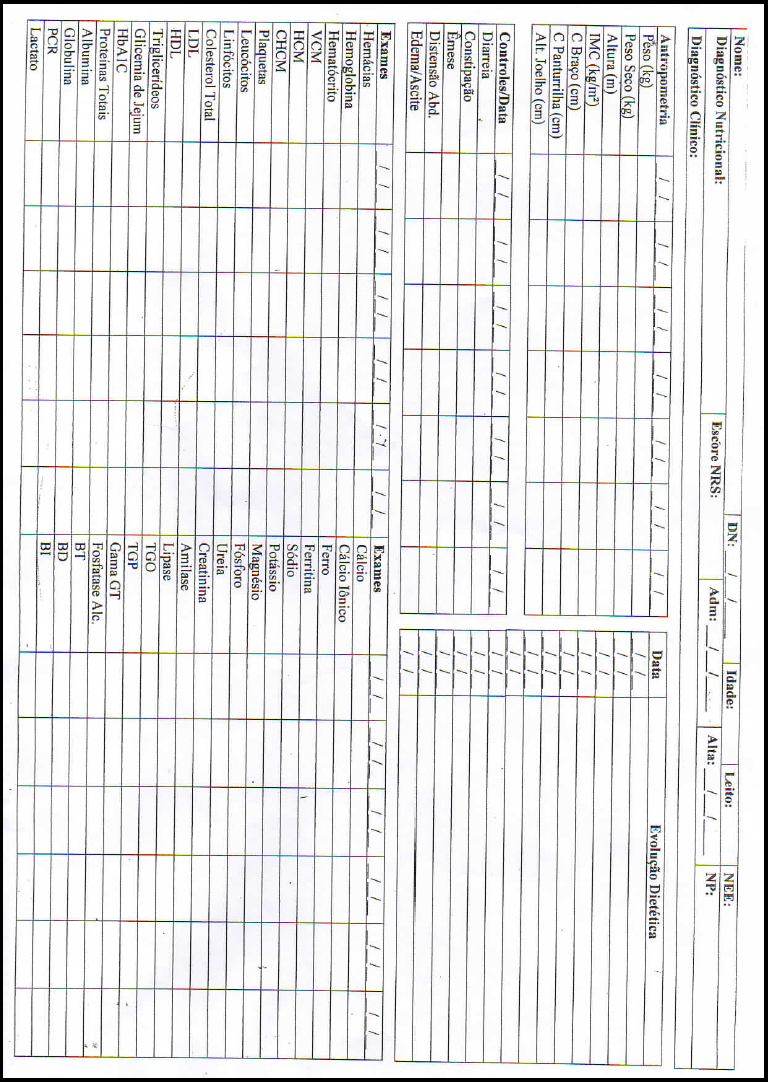
\includegraphics[scale=0.569]{Imagens/figura - formulario diagnostico clinico nutricional.png}
	\end{center}
	\legend{Fonte: \cite{huufs}.}
\end{figure}

Todos esses dados, antes de serem carregados no \textit{Data Warehouse} (DW) devem passar por um processo de ETL, que de forma sistemática realiza tratamento e limpeza dos dados advindos dos diversos arquivos fornecidos pela unidade de nutrição e pelo hospital. 

Um ponto importante a ser considerado, é que devido ao surto mundial de Sars-Cov-2, confirmado pela \citeonline{whocovid} em 2020, vários hospitais tiveram de passar por revisões dos seus protocolos de atendimento. Com a emissão de resolução do Conselho Federal de Nutrição e do Protocolo Operacional Padrão emitido pelo HU-UFS, a Unidade de Nutrição não mais realizou triagens nutricionais em pacientes de forma presencial e o acompanhamento nutricional foi realizado apenas de forma online e com regras diferentes para avaliação \cite{protocolocovidnutri, cfnutri646}. Com todas as mudanças ocorridas em 2020, a unidade não foi capaz de realizar o registro de alguns dados conforme padrão de anos anteriores e disponibilizou apenas a fonte de dados do ano de 2019 para consideração neste trabalho.

Com os dados disponíveis carregados no DW se faz necessário criar um modelo de dados OLAP, no qual as informações são organizadas conceitualmente em cubos de dados para análise dinâmica e multidimensional dos dados consolidados.

Com a possibilidade de consultas dinâmicas oferecidas pelo OLAP a Unidade de Nutrição Clínica solicitou além dos dados quantitativos também gráficos de comparação, composição e tendência para diferentes dimensões, sempre considerando uma visão de todo o hospital e uma visão por enfermaria como descritos abaixo: 

Para o indicador de Triagem Nutricional Realizada, as seguintes informações foram solicitados:
\begin{itemize}
    \item Quantidade de Triagens Nutricionais Realizadas ao Ano;
    \item Quantidade de Triagens Nutricionais Realizadas por Mês;
    \item Quantidade de Triagens Nutricionais Realizadas por Enfermaria ao Ano;
    \item Tendência de Triagens Nutricionais Realizadas por Enfermaria.
\end{itemize}

Para o indicador de Classificação de Risco foram solicitadas as seguintes informações:
\begin{itemize}
    \item Percentual de Classificação de Risco por Triagem Nutricional ao Ano;
    \item Percentual de Classificação de Risco por Triagem Nutricional detalhado por mês;
    \item Percentual de Classificação de Risco por Triagem Nutricional por Enfermaria ao Ano;
    \item Tendência de Classificação de Risco por Triagem Nutricional por Enfermaria detalhado por mês.
\end{itemize}

Para o indicador de Estado Nutricional foram solicitadas as seguintes informações:
\begin{itemize}
    \item Percentual do Estado Nutricional por Triagem Nutricional ao Ano;
    \item Percentual do Estado Nutricional por Triagem Nutricional detalhado por mês;
    \item Percentual do Estado Nutricional por Triagem Nutricional por Enfermaria ao Ano;
    \item Tendência do Estado Nutricional por Triagem Nutricional por Enfermaria detalhado por mês.
\end{itemize}

Para o indicador de Uso de Suplementação foram solicitadas as seguintes informações:
\begin{itemize}
    \item Quantidade de Pacientes em Uso de Suplemento;
    \item Quantidade de Pacientes em Uso de Suplemento por Enfermaria;
    \item Percentual de Uso de Suplementação por Triagem Nutricional ao Ano;
    \item Percentual de Uso de Suplementação por Triagem Nutricional por Enfermaria ao Ano;
    \item Tendência de Uso de Suplementação por Triagem Nutricional por Enfermaria detalhado por mês;
    \item Comparativo de pacientes que utilizam Suplementação com média de dias internado;
    \item Comparativo de pacientes que utilizam Suplementação com média de dias internado por enfermaria.
\end{itemize}

Para o indicador de Insumo foi solicitada a seguinte informação:
\begin{itemize}
    \item Percentual de Insumos utilizados por Enfermaria;
\end{itemize}

Para o indicador de Uso de Dieta Enteral foram solicitadas as seguintes informações:
\begin{itemize}
    \item Quantidade de Pacientes em Uso de Dieta Enteral;
    \item Quantidade de Pacientes em Uso de Dieta Enteral  por Enfermaria;
    \item Percentual de Uso de Dieta Enteral por Triagem Nutricional ao Ano;
    \item Percentual de Uso de Dieta Enteral por Triagem Nutricional por Enfermaria ao Ano;
    \item Tendência de Uso de Dieta Enteral por Triagem Nutricional por Enfermaria detalhado por mês;
    \item Comparativo de pacientes que utilizam Dieta Enteral com média de dias internado;
    \item Comparativo de pacientes que utilizam Dieta Enteral com média de dias internado por enfermaria.
\end{itemize}

Para o indicador de Complicações, que podem ocorrer por uso de suplementação e uso de dieta enteral foram solicitadas as seguintes informações:
\begin{itemize}
    \item Percentual de Complicações em Uso de Suplementação ao Ano;
    \item Percentual de Complicações em Uso de Suplementação por Enfermaria ao Ano;
    \item Percentual de Complicações em Uso de Dieta Enteral ao Ano;
    \item Percentual de Complicações em Uso de Dieta Enteral por Enfermaria ao Ano;
\end{itemize}

Para o indicador de Complicações, que podem ocorrer por Uso de Suplementação e Uso de Dieta Enteral foram solicitadas as seguintes informações:
\begin{itemize}
    \item Percentual de Complicações em Uso de Suplementação ao Ano;
    \item Percentual de Complicações em Uso de Suplementação por Enfermaria ao Ano;
    \item Percentual de Complicações em Uso de Dieta Enteral ao Ano;
    \item Percentual de Complicações em Uso de Dieta Enteral por Enfermaria ao Ano;
\end{itemize}

Para o indicador de Desfecho onde podem ocorrer altas, transferências ou óbitos, combinado a Dimensão de Classificações de Risco foram solicitadas as seguintes informações:
\begin{itemize}
    \item Percentual de Desfecho por Classificação de Risco ao Ano;
    \item Percentual de Desfecho por Classificação de Risco por Enfermaria ao Ano;
\end{itemize}

\section{Ambiente de \textit{Business Intelligence}}

O ambiente BI escolhido utilizou o conjunto de ferramentas \textit{Pentaho Community}, que são mantidas e disponibilizadas gratuitamente pela Hitachi Vantara©. O \textit{Pentaho Community} fornece um pacote de ferramentas completo para soluções BI. Para este trabalho foram utilizadas as seguintes ferramentas: \textit{Pentaho Data Integration, Pentaho Schema Workbench e Pentaho Business Analytics Platform}.

Alguns pré-requisitos são necessários para o bom funcionamento do ambiente. Foram instalados os seguintes softwares auxiliares: Java SE \textit{Runtime Environment} 8 \textit{update} 261, PostgreSQL 12.5, PG Admin 4.24 e SQL \textit{Power Arquitect} 1.0.8. Ainda nesta seção são descritas as etapas de modelagem multidimensional do \textit{Data Warehouse} e do \textit{Data Mart}, o processo de ETL, o mapeamento lógico do cubo de dados OLAP, as consultas e os resultados dos \textit{Dashboards}.

\subsection{Modelagem Multidimensional}
Ao analisar as características das informações solicitadas pela gestão da unidade de nutrição, considerando cada necessidade como um problema a ser resolvido, foi concebido do modelo multidimensional usando a estrutura \textit{star schema}. O esquema foi modelado com 13 dimensões (Hospital, Enfermaria, Tempo, Paciente, Classificação Nutricional, Estado Nutricional, Complicações, Triagem Realizada, Suplementação, Dieta Enteral, Insumos, Edema e Desfecho) e uma Fato (Nutrição). A \autoref{fig_modelagemdatawarehouse} mostra o modelo de dados do \textit{Data Warehouse} projetado neste trabalho.

\begin{figure}[htb]
	\caption{\label{fig_modelagemdatawarehouse}Modelo Multidimensional do Data Warehouse.}
	\begin{center}
	    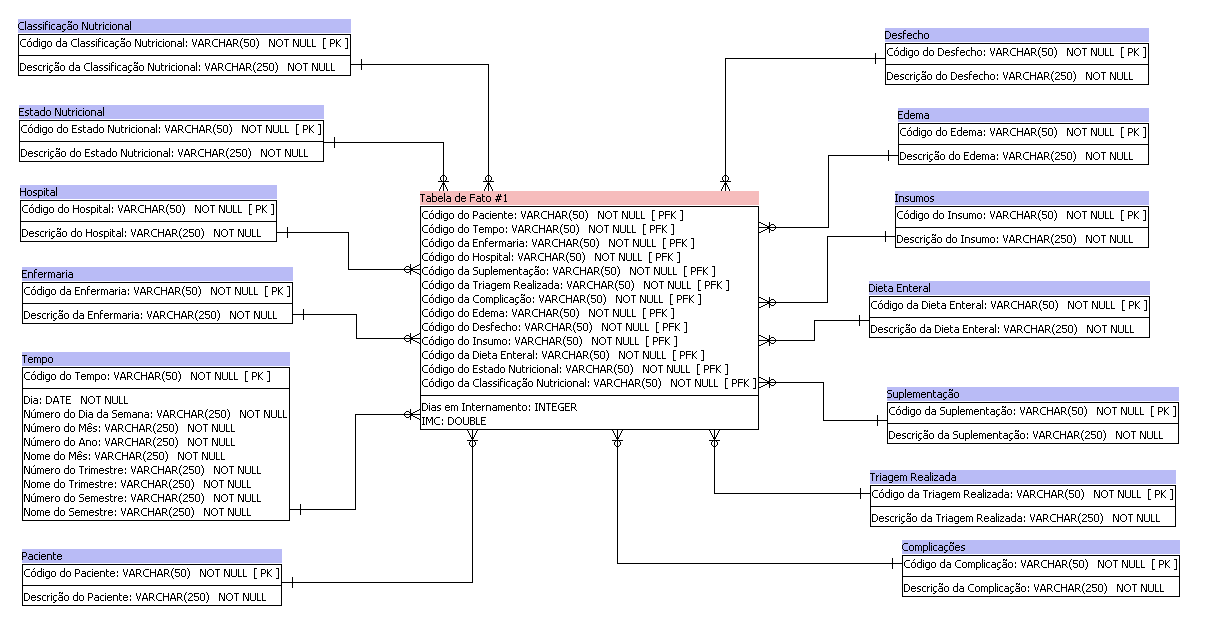
\includegraphics[scale=0.5]{Imagens/figura - modelagem multidimensional datawarehouse.png}
	\end{center}
	\legend{Fonte: Autor.}
\end{figure}

Com o objetivo de permitir melhor performance para as consultas também foi projetado um cubo OLAP de modelo relacional, mais especificamente chamado de \textit{Relational Online Analitycal Processing} (ROLAP), como é mostrado na \autoref{fig_modelagemdatamart}.

\newpage
\begin{figure}[htb]
	\caption{\label{fig_modelagemdatamart}Modelo Relacional do Data Mart.}
	\begin{center}
	    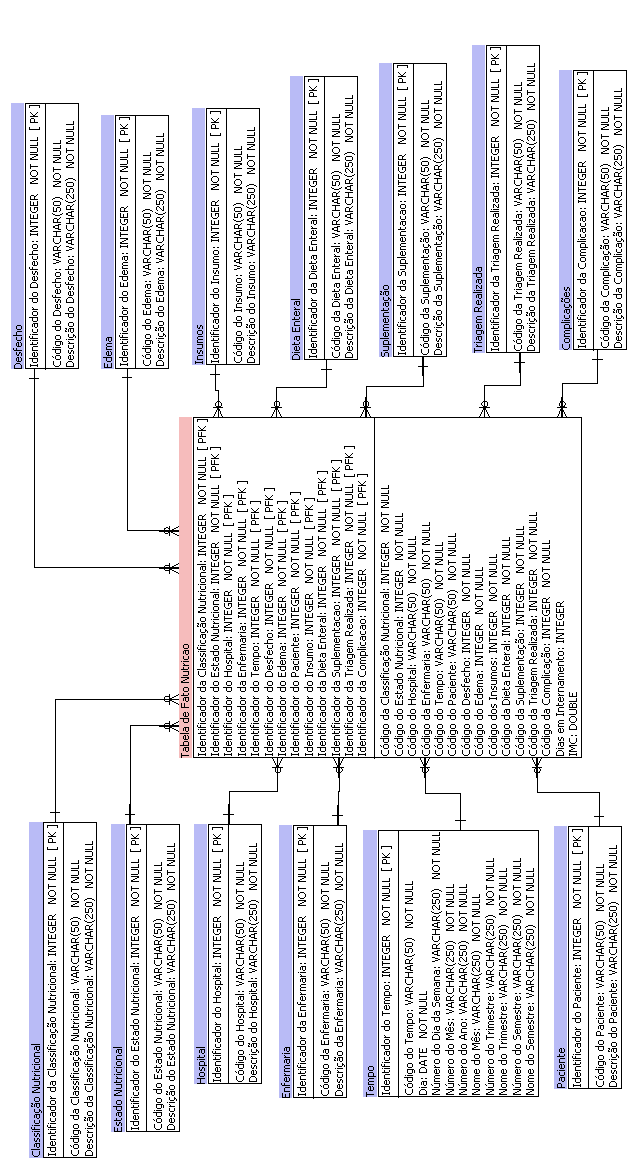
\includegraphics[scale=0.5]{Imagens/figura - modelagem multidimensional datamart.png}
	\end{center}
	\legend{Fonte: Autor.}
\end{figure}

O projeto multidimensional e o projeto do cubo ROLAP foram construídos com a ferramenta SQL \textit{Power Architect}, que além da concepção, auxilia na geração e execução do \textit{script} de criação tanto do \textit{Data Warehouse}, quanto do \textit{Data Mart}, implementados na sintaxe do PostgreSQL. Além de ser um SGBD robusto e gratuito, o PostgreSQL também é o sistema de gerenciamento de banco de dados utilizado pelo HU. 

\subsection{Processo de Extração, Transformação e Carga}
Com o modelo dimensional construído, foi dada sequência à próxima etapa do projeto, o desenvolvimento do processo de extração, transformação e carga. Para a fase de ETL foi utilizado o \textit{Pentaho Data Integration} (PDI), ferramenta da Pentaho utilizada para sistematizar o processo de tratamento e limpeza dos dados oriundos das fontes de dados e inserção nos armazéns de dados e nos \textit{Data Marts}.

A partir dos arquivos disponibilizados pela Unidade de Nutrição, em formato de arquivo de planilha no padrão Open XML adaptado pela Microsoft (XLSX), foram corrigidos, padronizados e tratados todos os desvios e inconsistências encontradas. Sequencialmente é iniciada a carga dos dados no DW, concluindo a persistência dos dados consolidados. Foram desenvolvidos um \textit{script} ETL para cada dimensão e um \textit{script} para a tabela de fato, resultando em 14 \textit{scripts} ETL. A seguir, estão as figuras das transformações utilizadas para a carga completa do DW. 
\newpage

\begin{figure}[htb]
	\caption{\label{fig_etldimensaohospital}Processo ETL para a Dimensão Hospital.}
	\begin{center}
	    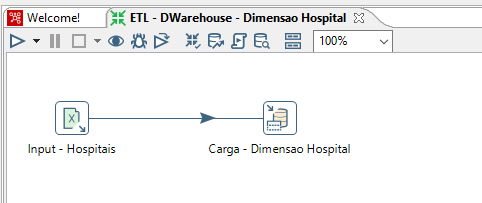
\includegraphics[scale=0.8]{Imagens/figura - etl dw hospital.png}
	\end{center}
	\legend{Fonte: Autor.}
\end{figure}

Na \autoref{fig_etldimensaoenfermaria} os dados relacionados as enfermarias do Hospital Universitário foram consultados do banco de dados do Aplicativo de Gestão para Hospitais universitários (AGHU). 
\begin{figure}[htb]
	\caption{\label{fig_etldimensaoenfermaria}Processo ETL para a Dimensão Enfermaria.}
	\begin{center}
	    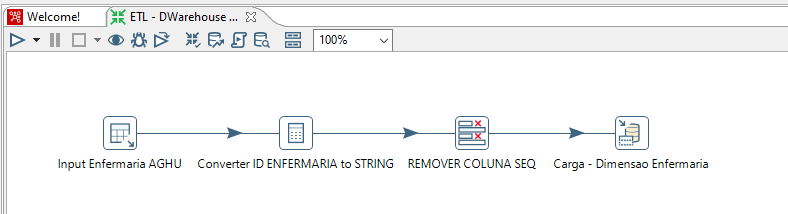
\includegraphics[scale=0.7]{Imagens/figura - etl dw enfermaria.png}
	\end{center}
	\legend{Fonte: Autor.}
\end{figure}

\begin{figure}[htb]
	\caption{\label{fig_etldimensaotriagem}Processo ETL para a Dimensão Triagem Realizada.}
	\begin{center}
	    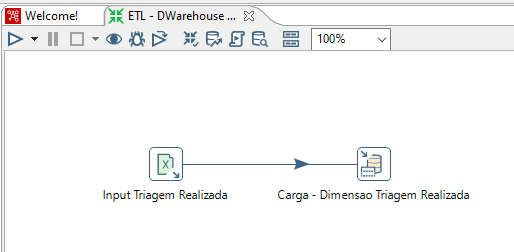
\includegraphics[scale=0.64]{Imagens/figura - etl dw triagem.png}
	\end{center}
	\legend{Fonte: Autor.}
\end{figure}

\begin{figure}[htb]
	\caption{\label{fig_etldimensaotempo}Processo ETL para a Dimensão Tempo.}
	\begin{center}
	    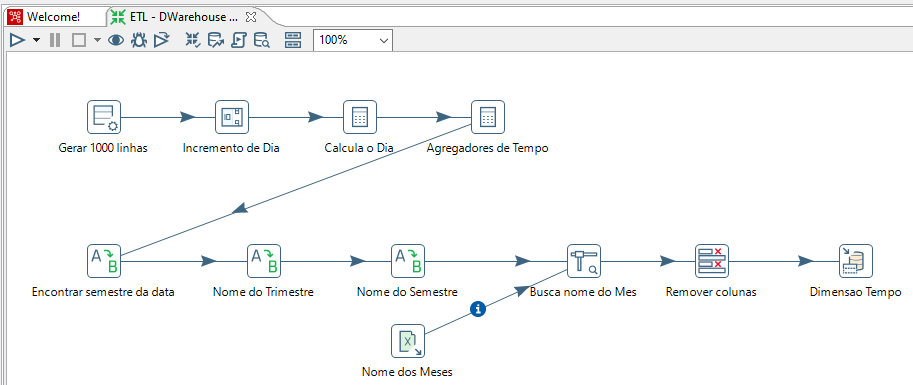
\includegraphics[scale=0.6]{Imagens/figura - etl dw tempo.png}
	\end{center}
	\legend{Fonte: Autor.}
\end{figure}

\begin{figure}[htb]
	\caption{\label{fig_etldimensaopaciente}Processo ETL para a Dimensão Paciente.}
	\begin{center}
	    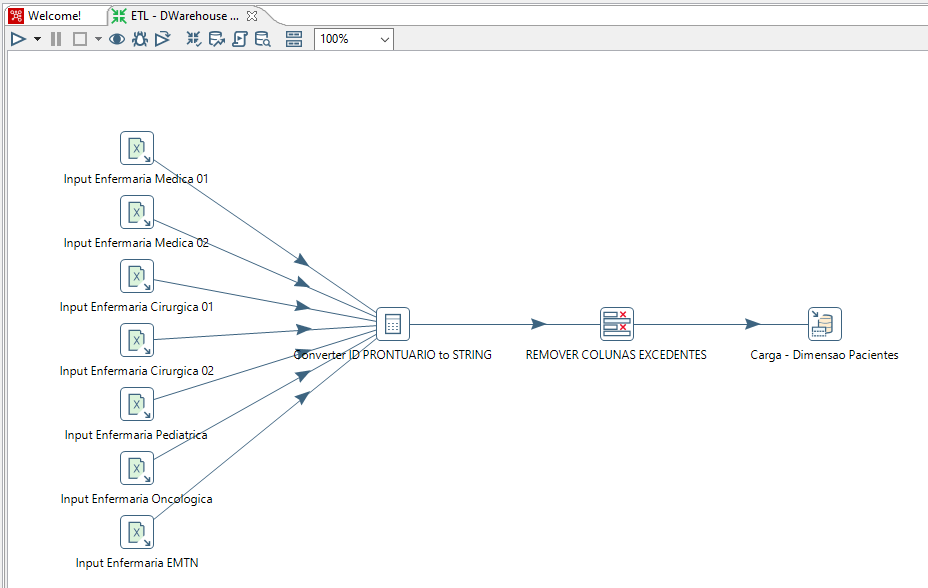
\includegraphics[scale=0.6]{Imagens/figura - etl dw paciente.png}
	\end{center}
	\legend{Fonte: Autor.}
\end{figure}

\begin{figure}[htb]
	\caption{\label{fig_etldimensaosuplementacao}Processo ETL para a Dimensão Suplementação.}
	\begin{center}
	    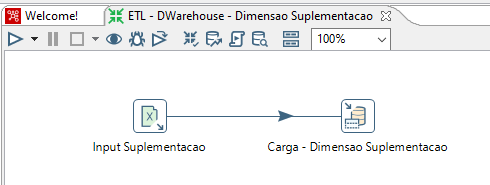
\includegraphics[scale=0.75]{Imagens/figura - etl dw suplementacao.png}
	\end{center}
	\legend{Fonte: Autor.}
\end{figure}

\begin{figure}[htb]
	\caption{\label{fig_etldimensaoinsumo}Processo ETL para a Dimensão Insumos.}
	\begin{center}
	    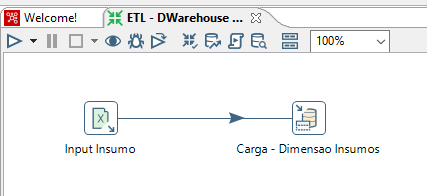
\includegraphics[scale=0.85]{Imagens/figura - etl dw insumos.png}
	\end{center}
	\legend{Fonte: Autor.}
\end{figure}

\begin{figure}[htb]
	\caption{\label{fig_etldimensaoestado}Processo ETL para a Dimensão Estado Nutricional.}
	\begin{center}
	    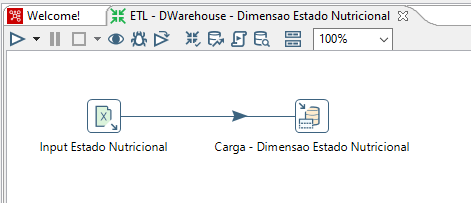
\includegraphics[scale=0.85]{Imagens/figura - etl dw estadonutricional.png}
	\end{center}
	\legend{Fonte: Autor.}
\end{figure}

tentaiva apos um texot.
\newpage
\subsection{Mapeamento e Consultas OLAP}
Schema Workbench Lorem impsum Lorem impsum Lorem impsum Lorem impsum Lorem impsum Lorem impsum Lorem impsum Lorem impsum Lorem impsum Lorem impsum Lorem impsum Lorem impsum Lorem impsum Lorem impsum Lorem impsum Lorem impsum Lorem impsum Lorem impsum Lorem impsum Lorem impsum Lorem impsum Lorem impsum Lorem impsum Lorem impsum Lorem impsum Lorem impsum Lorem impsum Lorem impsum Lorem impsum Lorem impsum Lorem impsum Lorem impsum Lorem impsum

 Lorem impsum Lorem impsum Lorem impsum Lorem impsum Lorem impsum Lorem impsum Lorem impsum Lorem impsum Lorem impsum Lorem impsum Lorem impsum Lorem impsum Lorem impsum Lorem impsum

\subsection{Ambiente de Relatórios}
Saiku Analytics Lorem impsum Lorem impsum Lorem impsum Lorem impsum Lorem impsum Lorem impsum Lorem impsum Lorem impsum Lorem impsum Lorem impsum Lorem impsum Lorem impsum Lorem impsum Lorem impsum Lorem impsum Lorem impsum Lorem impsum Lorem impsum Lorem impsum Lorem impsum Lorem impsum Lorem impsum Lorem impsum Lorem impsum Lorem impsum Lorem impsum Lorem impsum Lorem impsum Lorem impsum Lorem impsum Lorem impsum Lorem impsum Lorem impsum

 Lorem impsum Lorem impsum Lorem impsum Lorem impsum Lorem impsum Lorem impsum Lorem impsum Lorem impsum Lorem impsum Lorem impsum Lorem impsum Lorem impsum Lorem impsum Lorem impsum

\section{Resultados}
\subsection{Dashboards Obtidos}
Resultados Lorem impsum Lorem impsum Lorem impsum Lorem impsum Lorem impsum Lorem impsum Lorem impsum Lorem impsum Lorem impsum Lorem impsum Lorem impsum Lorem impsum Lorem impsum Lorem impsum Lorem impsum Lorem impsum Lorem impsum Lorem impsum Lorem impsum Lorem impsum Lorem impsum Lorem impsum Lorem impsum Lorem impsum Lorem impsum Lorem impsum Lorem impsum Lorem impsum Lorem impsum Lorem impsum Lorem impsum Lorem impsum Lorem impsum

 Lorem impsum Lorem impsum Lorem impsum Lorem impsum Lorem impsum Lorem impsum Lorem impsum Lorem impsum Lorem impsum Lorem impsum Lorem impsum Lorem impsum Lorem impsum Lorem impsum

% ---
% primeiro capitulo de Resultados
% ---
\chapter{Considerações Finais}
% ---

% ---
\section{Vestibulum ante ipsum primis in faucibus orci luctus et ultrices
posuere cubilia Curae}
% ---

\lipsum[21-22]

% ---
% segundo capitulo de Resultados
% ---
\chapter{Nam sed tellus sit amet lectus urna ullamcorper tristique interdum
elementum}
% ---

% ---
\section{Pellentesque sit amet pede ac sem eleifend consectetuer}
% ---

\lipsum[24]